\documentclass{article}

\usepackage[utf8]{inputenc}
\usepackage[T1]{fontenc}
\usepackage[czech]{babel}
\usepackage{mathtools}
\usepackage{amsmath}
\usepackage{dirtytalk}
\usepackage{graphicx}


\title{hello}
\author{EB2INE01}

\begin{document}

    \maketitle

\section{Segmentace}

\begin{itemize}
    \item Geografická
    \begin{itemize}
        \item Region - Globální trh
    \end{itemize}
    \item Demografická
    \begin{itemize}
        \item Věk - 16+
        \item Pohlaví - muži a ženy
        \item Fáze životního cyklu - Mladí a svobodní, Mladé páry, Full nest I a II
        \item Povolání - studenti, zaměstnanci, profesionálové
    \end{itemize}
    \item Behaviorální
    \begin{itemize}
        \item Loajalita - skalní loajální a loajální zákazníci
        \item Vyhledávané benefity - efektivita, přesnost, rychlost
        \item Osobnost - odhodlanost a abicióznost
        \item současný status užívání - neuživatelé, potenciální uživatelé, noví uživatelé, stálí uživatelé, ex-uživatelé
    \end{itemize}
    \item Psychografická
    \begin{itemize}
        \item Sociální třída - nižší třída, pracující třída, střední třída a vyšší třída
        \item Životní styl - Mainstreamer, Aspirer, Succeeder, Explorer, Reformer
    \end{itemize}
\end{itemize}

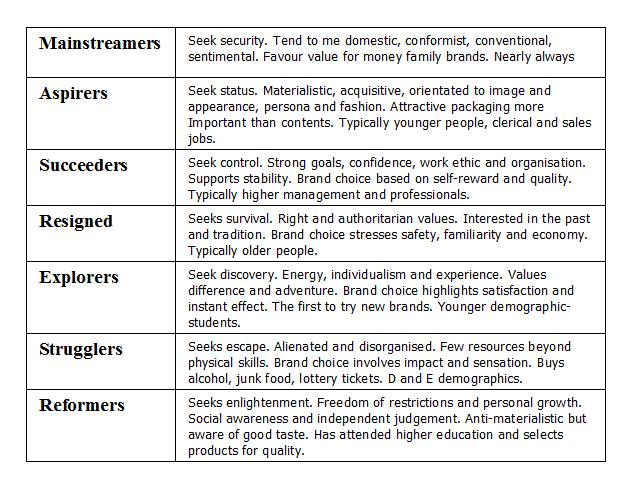
\includegraphics[width=\linewidth]{cross_cultural_consumer_characterization.jpg}

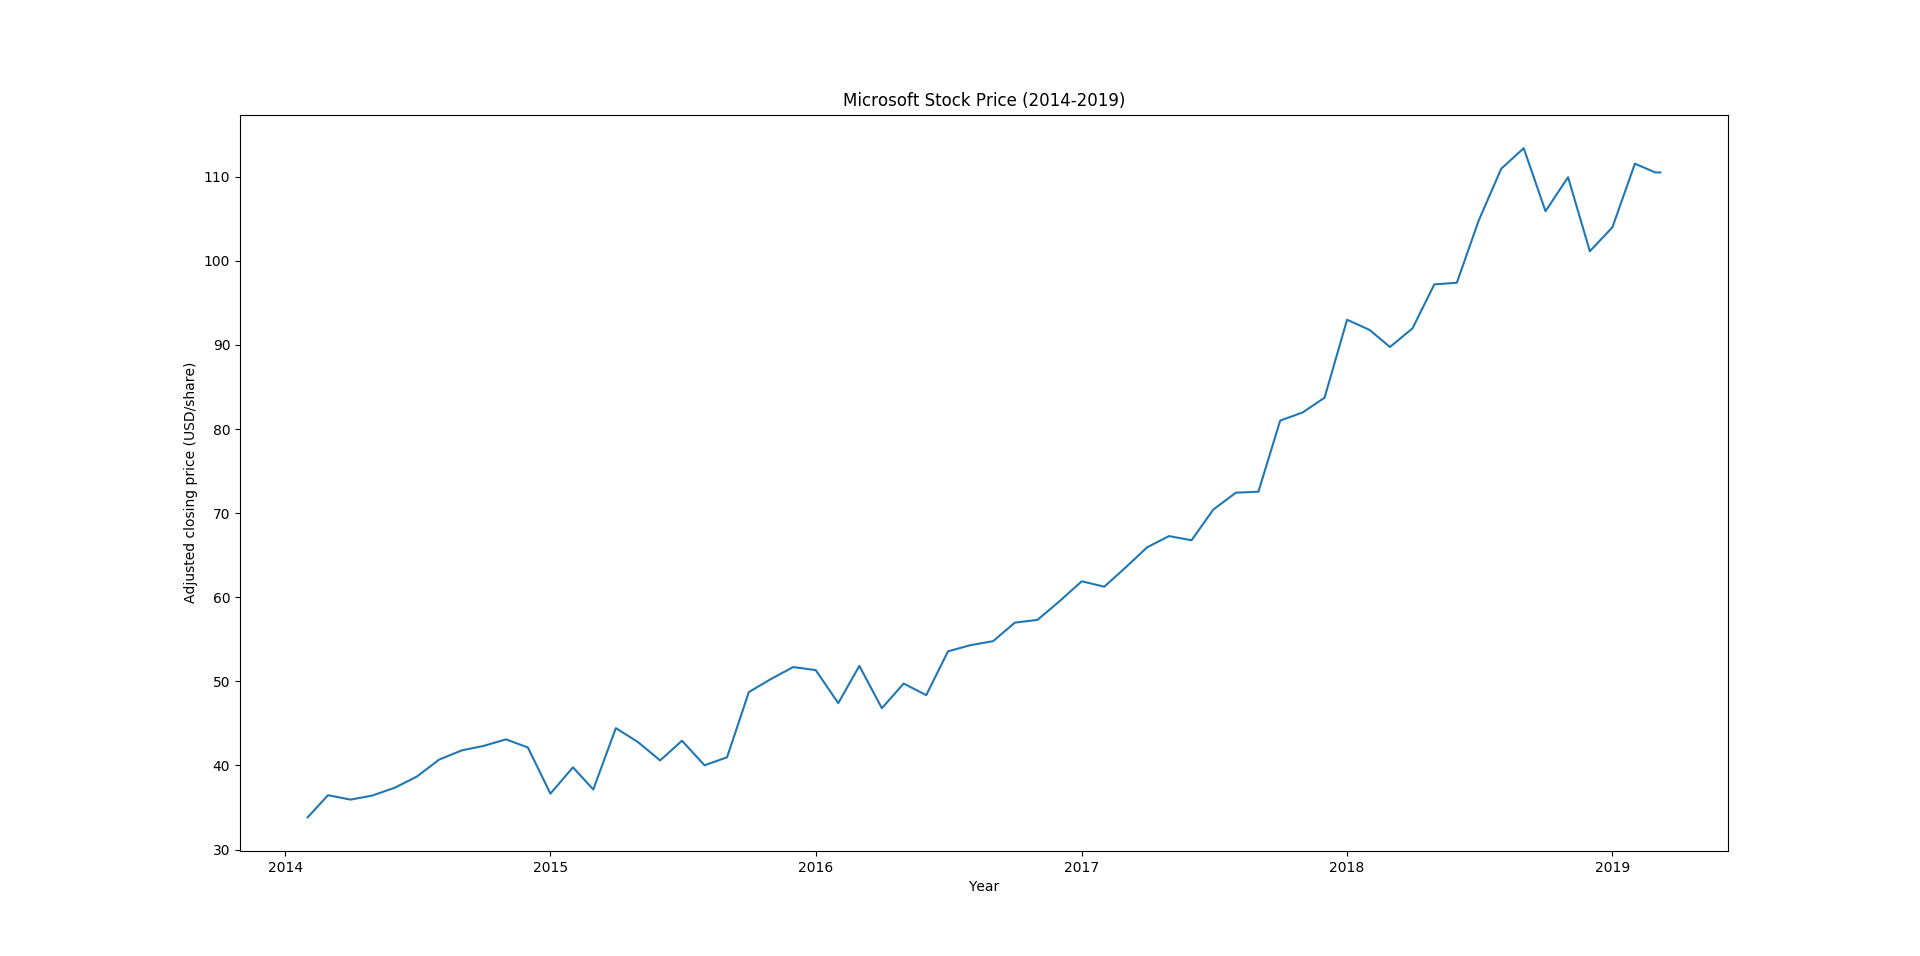
\includegraphics[width=\linewidth]{stock_price_2014_2019.png}


\section{Reakce firem}
Malé a střední firmy využívají služeb Microsoftu pro uskutečnění svého podnikatelského záměru. Při pronajmutí infrastruktury se šetří náklady na zřízení a údržbu, infrastruktura je flexibilní, takže její rozšíření je jen otázkou \say{několika kliků myší.} Cloudové služby (Office365) jsou zase přístupny všude, kde funguje počítač s prohlížečem, což v dnešní době je skoro samozřejmostí.

\section{Reakce konkurence}
Na trhu působí málo společností. Údržba datacenter je velice nákladná. Konkurence (Google, Amazon) se, stejně jako Microsoft, snaží zpřístupnit své nástroje co nejširší business veřejnost, stávající zákazníky si dlouhodobě udržovat nabízet jim nové produkty a zkvalitňovat ty staré, které jsou propojené s ekosystémem jejich značky. Zákazník je, potom, méně náchylný k přechodu ke konkurenci; přechod by byl zdlouhový a nepohodlný.

\section{Reakce zákazníků}
tbd

\section{Projevy v marketingovém mixu}
\begin{itemize}
    \item Produkt - Microsoft klade důraz na kvalitu a jednoduchost používání svých produtků. Hlavní prvek změny strategie je proměna výrobku ve službu
    \item Cena - Služby se platí periodicky, slevy jsou poskytovány při dlouhodobých závazcích a pro akademické subjekty (některé produkty jsou i zdarma za určitých podmínek)
    \item Propagace - Microsoft využívá jak tradičních masových médií, tak i svých již zavedených produktů (hlavně operačního systému Windows, skrze který může nabízet nové služby)
    \item Místo - produkt je dostupný přes internet
\end{itemize}



\end{document}
